\documentclass[11pt]{article}

\usepackage[margin=1.25in]{geometry}

\usepackage{amsmath}
\usepackage{amssymb}
\usepackage{graphicx}
\usepackage{amsfonts}
\usepackage{enumitem}
\usepackage{tikz}
\usetikzlibrary{positioning,calc,arrows,arrows.meta, shapes}


\begin{document}
	
	
	\title{Newtonian, Lagrangian and Hamiltonian mechanics are not equivalent}
	\author{Assumptions of Physics Collaboration}
	
	\date{}
	
	\maketitle
	
After taking a course in advanced mechanics, one is often left with the impression that Netwonian, Lagrangian and Hamiltonian particle mechanics are all equivalent. But is this the case?

If the three different mechanics are simply riformulations of one another, it should be true that we can express any system in all three. That is, for every expression of the force/Lagrangian/Hamiltonian we can find a suitable force/Lagrangian/Hamiltonian. Let's see if this can be done.

\section{Equation review}

We will look at the equations for a single particle in three dimensions. To make the notation consistent, we will use $q^i$, $\dot{q}^i$ and $\ddot{q}^i$ for position, velocity and acceleration, and follow Einstein notation.

A system is Netwonian if there is a mass $m$ and a force $F^i(q^j,\dot{q}^k)$ such that Newton's second law applies:
\begin{equation}
\label{Fma}
F^i=m\ddot{q}^i
\end{equation}

A system is Lagrangian if there is a function $L(q^i,\dot{q}^j)$ such that the system obeys the Euler-Lagrange equations:
\begin{equation}
\label{EulerLagrange}
 \frac{d}{dt} \frac{\partial L}{\partial \dot{q}^i} = \frac{\partial L}{\partial q^i}
\end{equation}

A system is Hamiltonian if there is a function $H(q^i,p_j)$ such that the system follows Hamilton's equations:
\begin{equation}
\begin{aligned}
\frac{dq^i}{dt} &= \frac{\partial H}{\partial p_i} \\
\frac{dp_i}{dt} &= - \frac{\partial H}{\partial q^i}
\end{aligned}
\label{Hamilton}
\end{equation}

In many cases, the same system admits all three descriptions. A free particle is such a system, as
\begin{equation}
\begin{aligned}
F^i&=0 \\
L&=\frac{1}{2}m|v|^2 \\
H&=\frac{1}{2}\frac{|p|^2}{m}
\end{aligned}
\end{equation}
yield the same trajectories. Is this true for all systems?

\section{The mathematical solution}
First of all, note that to specify a Newtonian system we need to specify three functions, one for each degree of freedom, while for a Hamiltonian and Lagrangian system we only need to specify one function. Also note that small changes of the forces, Lagrangian and Hamiltonian, induce small change in the equation of motion. Mathematically, there is no way to create a continuous one-to-one correspondence between vectors of three functions and single functions. This means that there are necessarily Newtonian systems that do not allow a Hamiltonian and Lagrangian formulations: there just aren't enough Lagrangians/Hamiltonians to do it!

What about the other direction: are there Lagrangian or Hamiltonian systems that do not allow Newtonian formulation? To do this, we have to write the equations of motion so that the acceleration is explicit. Let's start with Lagranian systems.

Using the chain rule, we expand the left side of \eqref{EulerLagrange}
\begin{align*}
	\frac{d}{dt} \left( \frac{\partial L}{\partial \dot{q}^i} \right) &= \frac{\partial}{\partial q^j} \left( \frac{\partial L}{\partial \dot{q}^i} \right) \frac{dq^j}{dt} + \frac{\partial}{\partial \dot{q}^k} \left( \frac{\partial L}{\partial \dot{q}^i} \right) \frac{d\dot{q}^k}{dt} \\
	&= \frac{\partial^2 L}{\partial q^j \partial \dot{q}^i} \dot{q}^j + \frac{\partial^2 L}{\partial \dot{q}^k \partial \dot{q}^i} \ddot{q}^k
\end{align*}
We can then rewrite the Euler-Lagrange equations as:
\begin{equation}
	\label{EulerLagrangeMod}
	\frac{\partial^2 L}{\partial \dot{q}^k \partial \dot{q}^i} \ddot{q}^k = \frac{\partial L}{\partial q^i} -  \frac{\partial^2 L}{\partial q^j \partial \dot{q}^i} \dot{q}^j
\end{equation}
Now we have the acceleration in the equation, but the equation is still implicit: on the left side, the acceleration is multiplied by the Hessian matrix of the Lagrangian. To make it explicit, we invert the matrix and write
\begin{equation}
	\label{EulerLagrangeExpl}
	 \ddot{q}^k = \left[ \frac{\partial^2 L}{\partial \dot{q}^k \partial \dot{q}^i} \right]^{-1} \left[ \frac{\partial L}{\partial q^i} -  \frac{\partial^2 L}{\partial q^j \partial \dot{q}^i} \dot{q}^j \right]
\end{equation}
The right side of the equation is a function of position and velocity, so we can identify it with the Newtonian force. However, we needed to assume that the determinant of the Hessian is different from zero
\begin{equation}
	\label{NonZeroHessian}
	\left| \frac{\partial^2 L}{\partial \dot{q}^k \partial \dot{q}^i} \right| \neq 0
\end{equation}
It would seem, then, that only Lagrangian system that satisfy condition \eqref{NonZeroHessian} are Newtonian, and therefore there are Lagrangian systems that are not Newtonian. However, if condition \eqref{NonZeroHessian} fails, Lagrangian mechanics fails to yield a unique solution. For example, if we set $L=0$, the action on all paths is the same, so action is stationary for all paths. The Euler-Lagrange equations simply become the identity $0=0$. Since the principle of stationary action is not well posed in these cases, we do not consider them proper Lagrangian systems, and therefore we conclude that all Lagrangian systems are Newtonian systems.

Let us now turn to Hamiltonian mechanics. The first set of equation in \eqref{Hamilton} tells us
\begin{equation*}
	\dot{q}^i = \frac{\partial H}{\partial p_i}
\end{equation*}
Using the chain rule, we have
\begin{align*}
	\ddot{q}^i &= \frac{d}{dt} \dot{q}^i  = \frac{d}{dt} \left( \frac{\partial H}{\partial p_i} \right) =  \frac{\partial}{\partial q^j} \left( \frac{\partial H}{\partial p_i} \right) \frac{dq^j}{dt} + \frac{\partial}{\partial p_k} \left( \frac{\partial H}{\partial p_i} \right) \frac{dp_k}{dt} \\
	&= \frac{\partial^2 H}{\partial q^j \partial p_i} \frac{\partial H}{\partial p_j} - \frac{\partial^2 H}{\partial p_k \partial p_i} \frac{\partial H}{\partial q^k}
\end{align*}
In this case, the acceleration is already explicit for all Hamiltonians. However, it is in general a function of position and momentum, while the Newtonian force must be expressed in terms of position and velocity. Hamilton's equation always give us the velocity as an explicit function of position and momentum, which is invertible if the Jacobian determinant is not zero
\begin{equation}\label{HamiltonianKE}
	\left| \frac{\partial q^i}{\partial p_j} \right| = \left| \frac{\partial^2 H}{\partial p_j \partial p_i} \right| \neq 0.
\end{equation}
Since Hamilton's equations are first order, all Hamiltonians lead to a well-posed problem. Therefore, in this case, there will be Hamiltonian systems that do not admit a Newtonian description. Moreover, given a Hamiltonian we can define the Lagrangian $L=p_i \dot{q}^i - H$ which, under condition \eqref{HamiltonianKE}, can be expressed as a function of position and velocity. Therefore, all Hamiltonian systems that can be expressed as Newtonian systems are also Lagrangian systems.

Our findings are summarized by the following diagram.

\begin{center}
	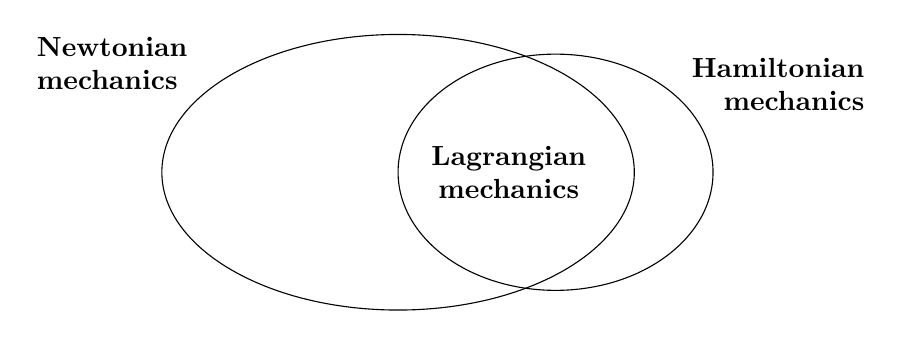
\begin{tikzpicture}
		\node[ellipse, draw, minimum width=6cm, minimum height=3.5cm, align=center, inner xsep=-2mm] (Newt) {};
		\node[ellipse, draw, minimum width=4cm, minimum height=3cm, align=center, inner xsep=-2mm] (Ham) at ([xshift=2cm]Newt) {};
		\node[align=left, above left] at (Newt.160) {\textbf{Newtonian}\\\textbf{mechanics}};
		\node[align=center, right] at ([xshift=0.3cm]Newt) {\textbf{Lagrangian}\\\textbf{mechanics}};
		\node[align=right, above right] at ([xshift=-0.2cm]Ham.20) {\textbf{Hamiltonian}\\\textbf{mechanics}};
	\end{tikzpicture}
\end{center}

\section{The physical significance}

The previous findings leave some questions open. First of all, what are the Newtonian systems that are not Lagrangian and Hamiltonian? What are the Hamiltonian systems that are not Newtonian and Lagrangian? Moreover, why do we move away from Newtonian mechanics, which seems to be able to describe many more systems than Lagrangian mechanics? What do we gain and what do we lose?

To answer these question, it is useful to distinguish between the kinematics of the system (i.e. its trajectory in space as described by position and velocity) and the dynamics of the system (i.e. the state of the system and the causes of motion, described by energy and momentum). Because observers can be in relative motion with each other, the kinematics is, in general, not enough to reconstruct the dynamics. For example, if you see a body decelerating, it could be either because a force is being applied to the body, or because a force is being applied to you. The trajectory, by itself, is not enough to distinguish what forces are acting on the system.

While the work of Galileo concentrated on the description of motion, the kinematics, Newton investigated the causes of motion, the dynamics. But Newtonian theory is still a kinematic theory: everything is in terms of position and velocity. It is the idea of inertial observer that allows us to distinguish which motions are really caused by something external, a ``real'' force, and which are due to change of coordinates, an ``apparent'' force. Therefore someone in an inertial frame can tell whether a body is decelerating because of an external force, whether a force is conservative or not and so on. The downside is that $F=ma$ is valid only in an inertial frame, and needs to be modified when not in an inertial frame by adding the correct inertial forces. 

Lagrangian and Hamiltonian mechanics take a different approach. In both frameworks the equations are the same for all observers. Therefore we are free to use whatever coordinates are the most useful for the system we are studying. In this sense, they are more general. The downside is that we have just one set of equations for all observers, inertial or not, and we are not going to be able to tell apart the ``real'' forces from the ``apparent'' forces. To compensate, both Hamiltonian and Lagrangian mechanics are restricted to those cases where the systems are isolated, in the sense that energy can't leave or enter the system, all forces are conservatives. This restriction allows us to reconstruct the dynamics from the kinematics.

Lagrangian and Hamiltonian mechanics, then, can describe only a subset of kinematic systems, those that do not have dissipative (or driving) forces, but use the same equations for all observers. Newtonian mechanics can describe all systems, but needs a different set of equation for different observers.

We have also seen that not all Hamiltonian systems are Newtonian, and the reason is because the momentum cannot be expressed as a function of velocity. There are very few of these, and the most physically significant is that of the photon taken as a particle. 

The Hamiltonian for a photon is
\begin{equation*}
H = c|p|.
\end{equation*}
The equations of motion are
\begin{align*}
\frac{dx}{dt} &= \frac{\partial H}{\partial p} = c \frac{\partial |p|}{\partial p} = c \frac{|p|}{p} \\
\frac{dp}{dt} &= - \frac{\partial H}{\partial x} = 0
\end{align*}
The momentum cannot be zero, since $H$ is discontinuous there. The velocity is $c$ in the direction of momentum, and therefore it hold no information about the momentum absolute value. If we just look at the trajectory of the photon, then, we are not able to reconstruct its momentum and therefore the velocity is not enough to tell us the full state of the system. Because of this, the photon as a particle is not a Langrangian or Newtonian system, but it is still a Hamiltonian one.

\section{Conclusion}

To sum it up, Netwonian, Lagrangian and Hamiltonian are not equivalent. Newtonian and Lagrangian systems are restricted to those for which the dynamics of the system (i.e. the causes of motion) is fully captured by the kinematics (i.e. the description of the motion). Lagrangian and Hamiltonian systems, on the other hand, are restricted to conservative systems, where no energy and no information is exchanged with the outside, where isolation holds and the system is deterministic and reversible.


\end{document}
